\documentclass[tikz,border=3pt]{standalone}
\usepackage[utf8]{inputenc}
\usepackage[T1]{fontenc}
\usepackage{lmodern}
\renewcommand{\familydefault}{\sfdefault}
\usepackage{sansmath}\sansmath
\usepackage{chemfig}
\usepackage{pgfplots}\pgfplotsset{compat=1.18,/pgf/number format/use comma,/pgf/number format/1000 sep={.}}
\usetikzlibrary{arrows.meta,calc,positioning,decorations.pathmorphing,patterns}
% paleta del sitio
\definecolor{nar}{HTML}{E8680C}\definecolor{narc}{HTML}{FFB35C}\definecolor{hielo}{HTML}{FFF3E8}
\definecolor{tinta}{HTML}{1D1D1F}\definecolor{gris}{HTML}{6E6E73}\definecolor{lila}{HTML}{7C5CF0}
\definecolor{azul}{HTML}{2F6FD6}\definecolor{menta}{HTML}{17A673}\definecolor{coral}{HTML}{E8342A}
\begin{document}
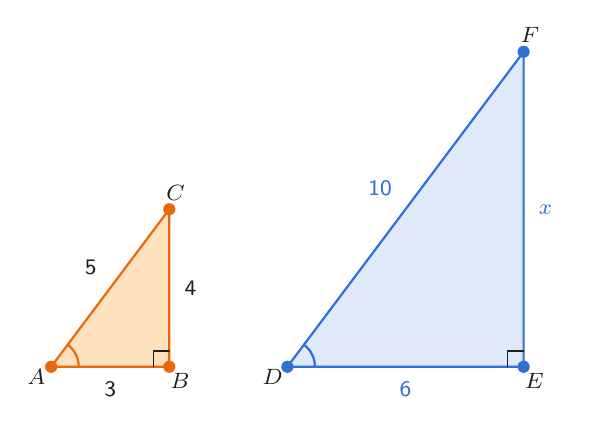
\begin{tikzpicture}[font=\small,x=0.5cm,y=0.5cm,line cap=round,line join=round,step={(1,1)}]
\filldraw[fill=narc!40,draw=nar,thick] (0,0)--(3,0)--(3.0,4.0)--cycle;
\fill[nar] (0,0) circle (2.2pt);
\node[font=\footnotesize,text=tinta,inner sep=0pt] at ($(0,0)+(-146:0.45)$) {$A$};
\fill[nar] (3,0) circle (2.2pt);
\node[font=\footnotesize,text=tinta,inner sep=0pt] at ($(3,0)+(-53:0.45)$) {$B$};
\fill[nar] (3.0,4.0) circle (2.2pt);
\node[font=\footnotesize,text=tinta,inner sep=0pt] at ($(3.0,4.0)+(69:0.45)$) {$C$};
\filldraw[fill=azul!15,draw=azul,thick] (6,0)--(12,0)--(12.0,8.0)--cycle;
\fill[azul] (6,0) circle (2.2pt);
\node[font=\footnotesize,text=tinta,inner sep=0pt] at ($(6,0)+(-146:0.45)$) {$D$};
\fill[azul] (12,0) circle (2.2pt);
\node[font=\footnotesize,text=tinta,inner sep=0pt] at ($(12,0)+(-53:0.45)$) {$E$};
\fill[azul] (12.0,8.0) circle (2.2pt);
\node[font=\footnotesize,text=tinta,inner sep=0pt] at ($(12.0,8.0)+(69:0.45)$) {$F$};
\path (0,0)--(3,0) node[midway,below=2pt,font=\footnotesize,text=tinta] {3};
\path (3,0)--(3.0,4.0) node[midway,right=2pt,font=\footnotesize,text=tinta] {4};
\path (0,0)--(3.0,4.0) node[midway,above left=2pt,font=\footnotesize,text=tinta] {5};
\path (6,0)--(12,0) node[midway,below=2pt,font=\footnotesize,text=azul] {6};
\path (12,0)--(12.0,8.0) node[midway,right=2pt,font=\footnotesize,text=azul] {$x$};
\path (6,0)--(12.0,8.0) node[midway,above left=2pt,font=\footnotesize,text=azul] {10};
\draw[tinta] (2.6,0)--(2.6,0.4)--(3,0.4); \draw[tinta] (11.6,0)--(11.6,0.4)--(12,0.4);
\draw[nar,thick] (0.7,0) arc (0:53.13:0.7); \draw[azul,thick] (6.7,0) arc (0:53.13:0.7);
\end{tikzpicture}
\end{document}
